\documentclass{article}
\usepackage[utf8]{inputenc}
\usepackage[russian]{babel}
\usepackage{graphicx}

\title{homeWork#3}
\author{Kalinina Ksenia A-13a-19}
\date{May 2022}

\begin{document}

\maketitle

\section{Задание №1. Реализуйте машины Тьюринга, которые позволяют выполнять следующие операции:}

1. Сложение двух унарных чисел

Алгоритм: 
Сначала идем до плюса и удаляем его, вместо него пишем 1, идем в конец, удаляем единицу и возвращаемся в начало

Например, 111+11 -> 111111 -> 11111

          1+111 -> 11111 -> 1111 


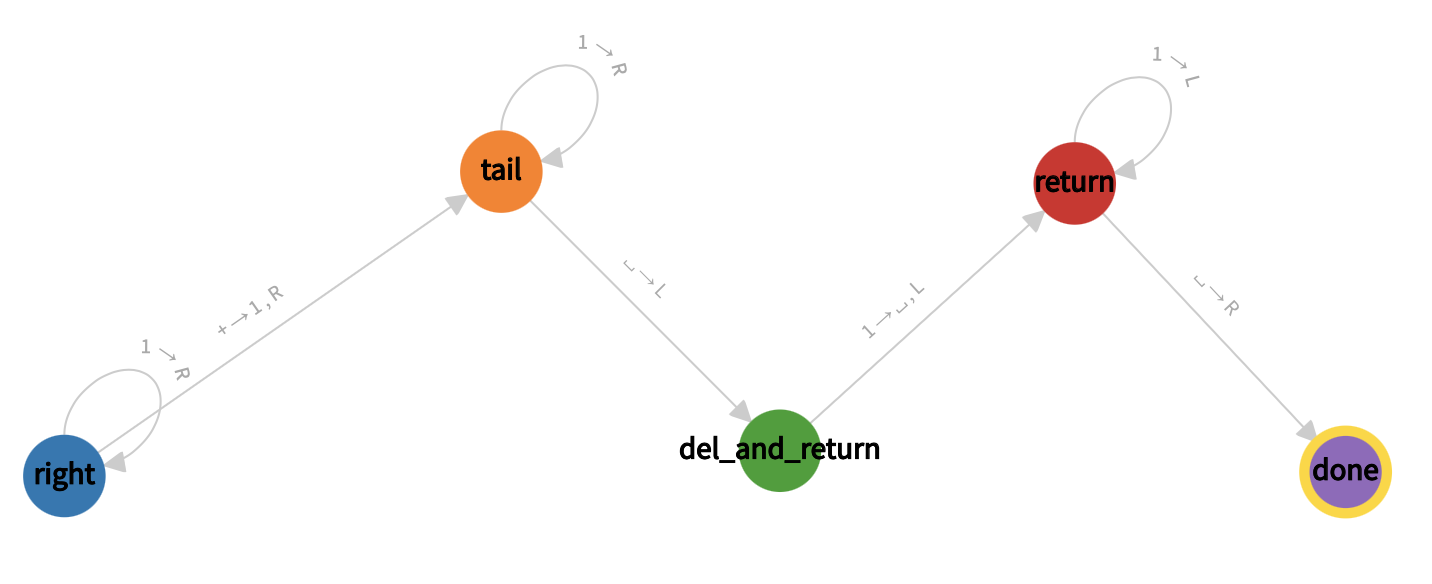
\includegraphics[weight = 13cm, height = 5cm]{1_1.png}


 2. Умножение двух унарных чисел
 
Алгоритм:
Сначала идем в конец и пишем знак '='; Далее идем к первому множителю и зануляем одну единичку, далее идем ко второму множителю и переписываем его после знака '=', как признак переноса цифры используем 0; Когда весь второй множитель перенесен за знак равенства, превращаем все нули второго множителя в единички. Далее идем к первому множителю и зануляем следующую единицу. Цикл повторяется до тех пор, пока первый множитель весь не занулится. Потом превращаем все нули первого множителя в единички. Готово.

Например, 11*11 -> 11*11= -> 01*11= -> 01*01=1 -> 01*00=11 -> 01*11=11 -> 00*11=11 -> 00*01=111 -> 00*00=1111 -> 00*11=1111 -> 11*11=1111


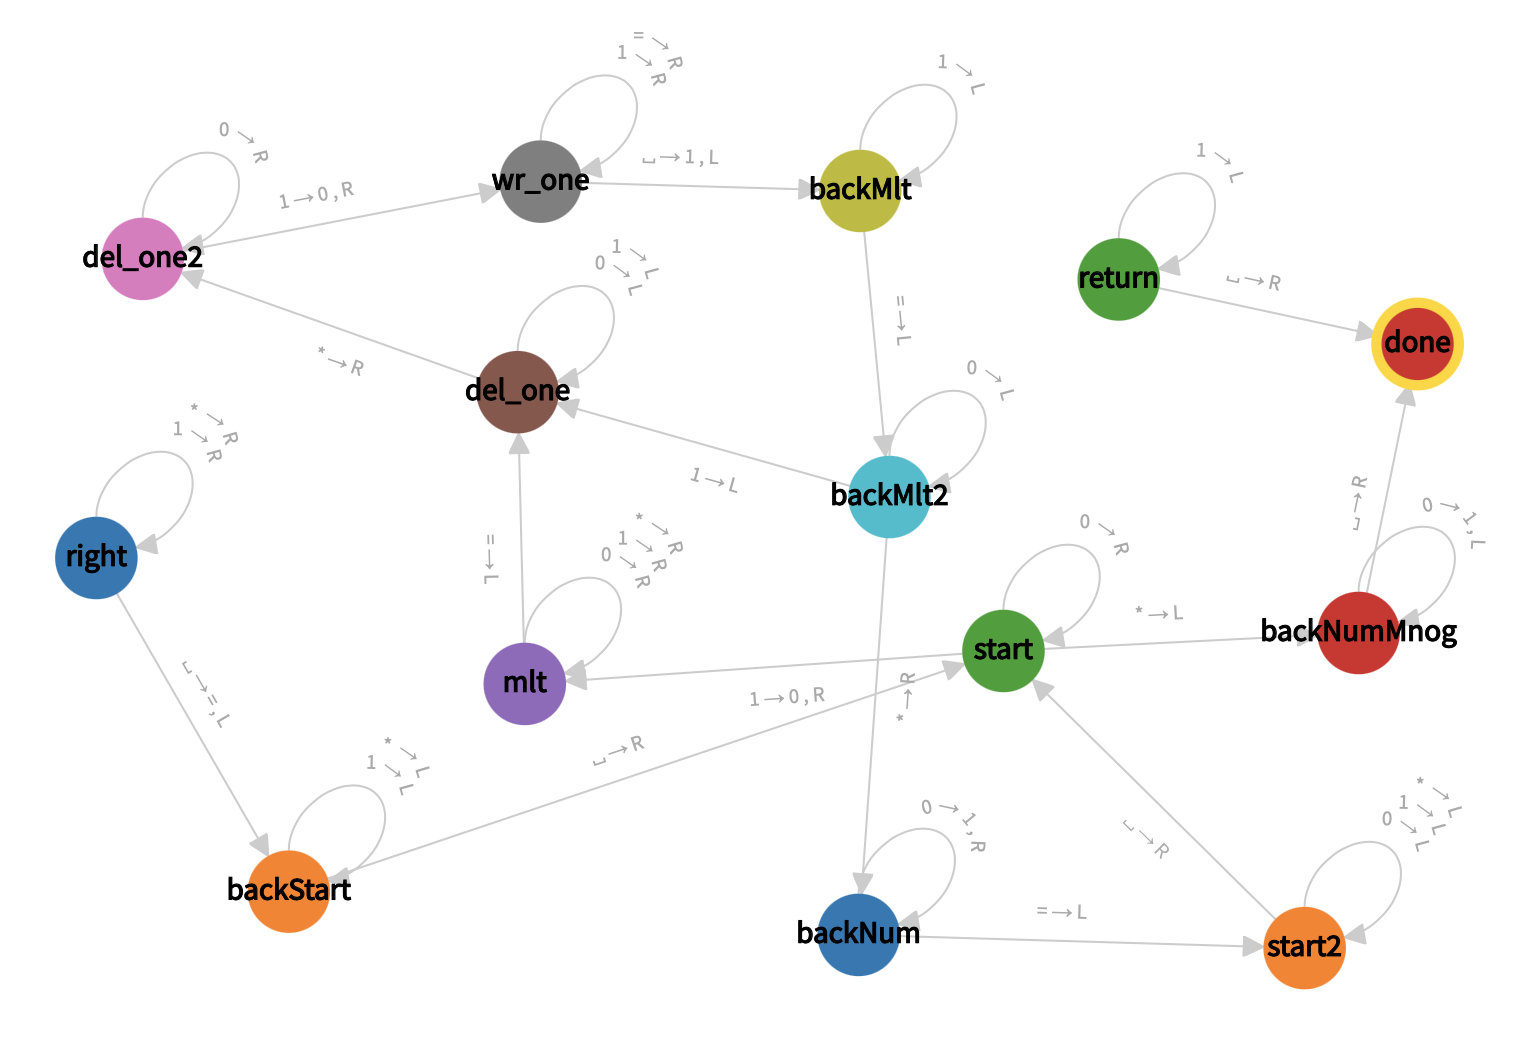
\includegraphics[weight = 25cm, height = 10cm]{1-2.png}


\section{Задание №2. Реализуйте машины Тьюринга, которые позволяют выполнять следующие операции:}

1. Принадлежность к языку \(L = \{0^n1^n2^n\}, n \geq 0\)

Алгоритм:
Преобразуем один ноль, одну единицу и одну двойку в буквы a, b, c соответсвенно. Далее повторяем этот цикл и идем на проверку, если встречается какая-то лишняя цифра, то МТ останавливается. Если все в порядке, то перед словом поставим !, как признак принадлежности слова к языку L.
Для n = 0, проверяем набор из 111

Например, 001122 -> a0b1c2 -> aabbcc -> !aabbcc
\newline
        0011222 ->  a0b1c22 -> aabbcc2 -> aabbcc2 // stop
\newline
        111 -> 111!

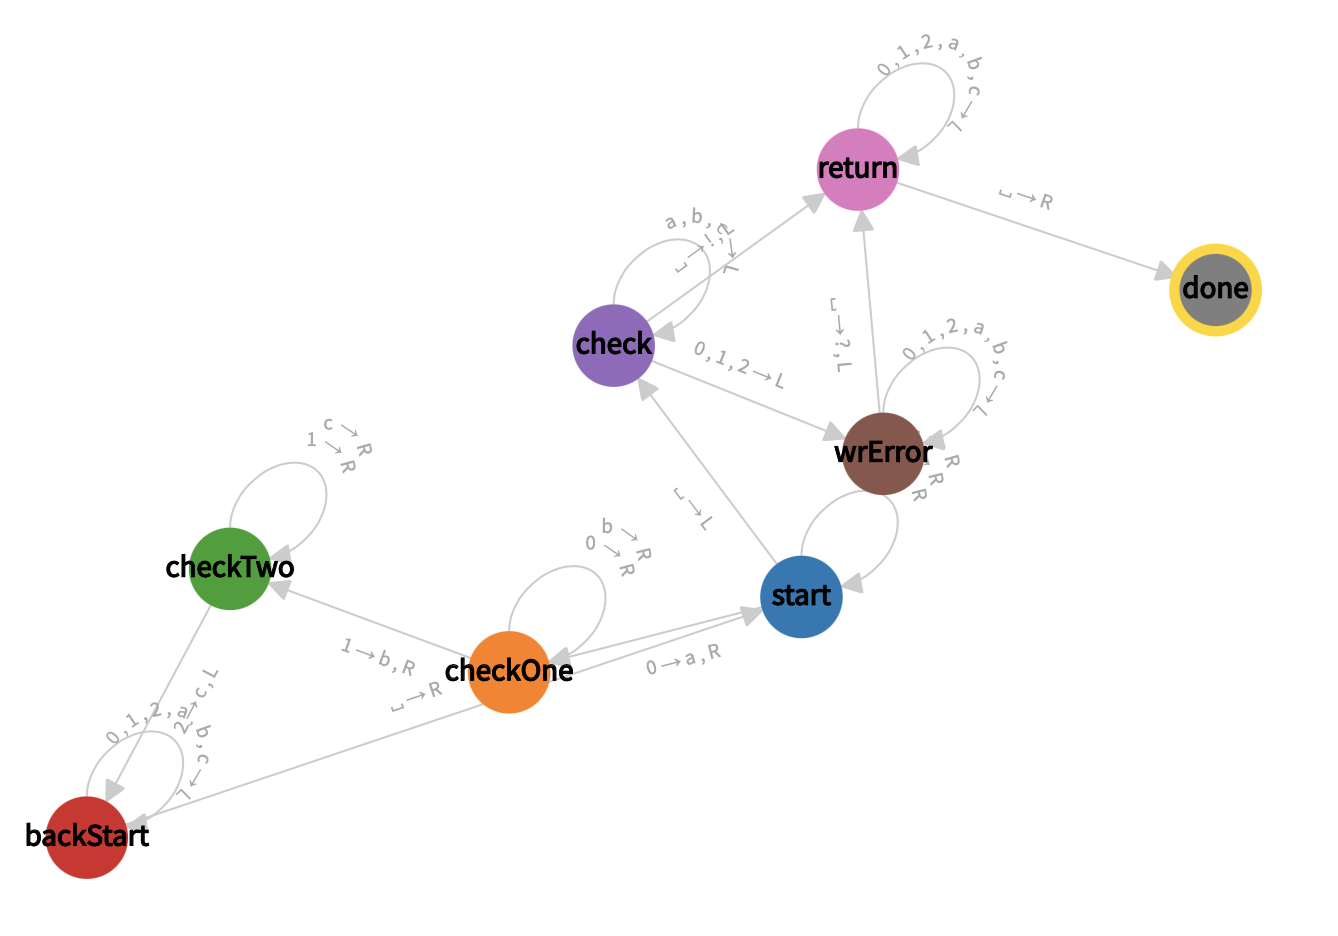
\includegraphics[weight = 25cm, height = 10cm]{2-1.png}


2. Проверка соблюдений правильности скобок в строке (минимум 3 вида скобок)

Алгоритм:
Ищем закрывающуюся скобку, меняем ее на х, идем в начало и ищем открывающуюся скобку того же вида, меняем ее на х. Далее возвращаемся в начало и повторяем цикл. Когда все скобки (парные) преобразованы в х, стираем их и ставим 1, как признак принадлежности языку. Если есть мы не нашли открывающуюся скобку того же вида, то ставим 0, как признак непринадлежности языку,

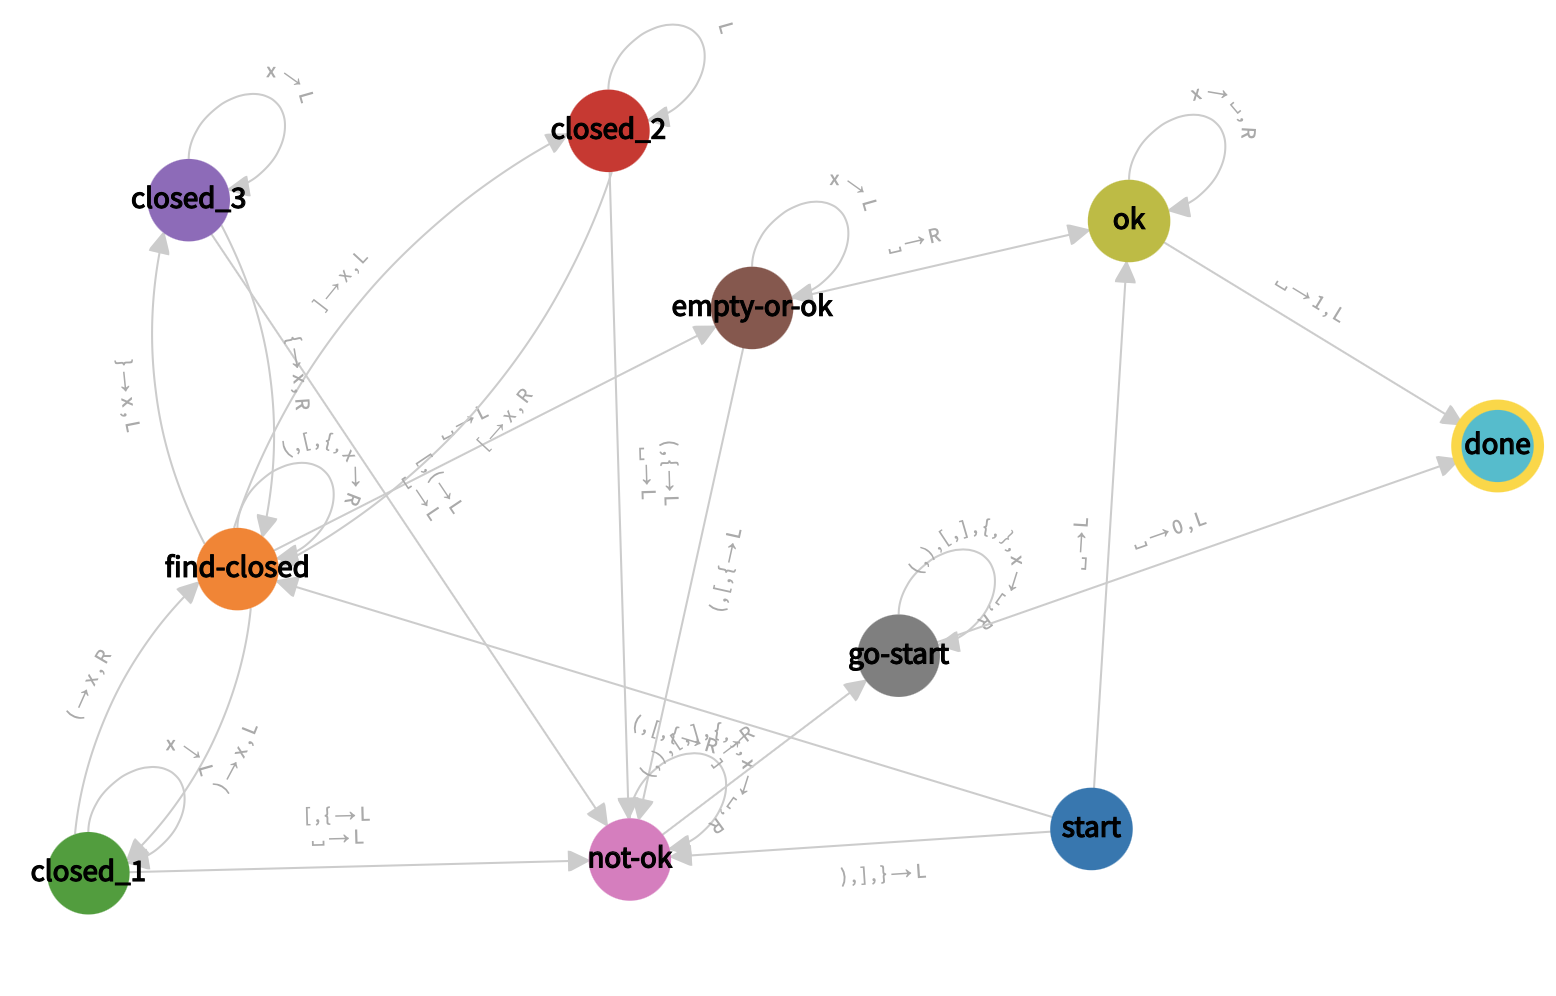
\includegraphics[weight = 25cm, height = 10cm]{2-2.png}

\end{document}
